\section{Анализ литературных источников, прототипов и формирование требований к проектируемому программному средству}
\label{sec:analysis}

Успех программного проекта во многом определяется на этапе подготовки, которая проводится с учетом всех особенностей проекта.

Первое предварительное условие, которое нужно выполнить перед конструированием, -- ясное формулирование проблемы, которую система должна решать.
Снижение риска является одной из основных целей подготовки: качественное планирование позволяет исключить главные аспекты риска на самых ранних стадиях работы.

Главный факторы риска в создании программного обеспечения — неудачная выработка требований.
Требования подробно описывают, что должна делать программная система.
Внимание к требованиям помогает свести к минимуму изменения системы после начала разработки~\cite{code_complete}.

Перед формулированием требований необходимо изучить ряд вопросов, которые напрямую влияют на все дальнейшие этапы разработки.
В частности, необходимо рассмотреть основные компоненты учёта персонального бюджета, методики и подходы оптимизации расходов, приемущества и недостатки целевой платформы.
По результатам анализа можно будет составить техническое задание к проектируемому программному средству, которое станет основой для составления функциональных требований.

\subsection{Аналитический обзор литературных источников}
\label{sec:analysis:literature}

Далее приводится анализ сведений, которые влияют на формулирование требований, дальнейшее проектирование и разработку программного средства.

\subsubsection{} Обзор основных составляющих персонального бюджета
\label{sec:analysis:literature:components}

% TODO: Add budget components overview

\subsubsection{} Обзор подходов по учёту доходов и расходов
\label{sec:analysis:literature:tracking}

% TODO: Add income/expense tracking overview

\subsubsection{} Обзор методик оптимизации расходов
\label{sec:analysis:literature:optimization}

% TODO: Add expense optimization overview

\subsubsection{} Анализ операционной системы Android в качестве целевой платформы
\label{sec:analysis:literature:android}

% TODO: Add android analysis (statistics, drawbacks and advantages)

\subsection{Обзор существующих прототипов и аналогов}
\label{sec:analysis:analogues}

Для решения проблемы учёта доходов и расходов разработано большое количество различных приложений, которые включают в себя:
\begin{itemize}
    \item решения для персональных компьютеров с операционной системой Windows;
    \item веб-приложения;
    \item мобильные приложения на платформах \andro и iOS\@.
\end{itemize}

Учитывая, что в рамках дипломного проектирования предполагается разработать приложение для платформы \andro, рассматриваться будут только существующие аналоги для данной платформы.

В магазине мобильных приложений для платформы \andro, \emph{Google Play}, представлены сотни приложений данной тематики, однако невозможно оценить точное число таких приложений из-за того, что \emph{Google Play} не предоставляет никакой общей статистики по количеству приложений.
Но даже по такому числу приложений можно сказать, что их данная тематика является популярной и востребованной.
В то же время можно сделать вывод, что до сих пор не появилось доминирующего приложения, каждое решает проблему по-своему.

Достаточно важным критерием среди мобильных приложений является качество и проработанность пользовательского интерфейса.

Универсальной метрики, позволяющей оценить удобство использования и качество пользовательского интерфейса, нет.
Однако, в 2014 году компания Google представила набор рекомендаций по правильному, с их точки зрения, оформлению пользовательского интерфейса под названием <<Material Design>>~\cite{google_material_news}.
Данные рекомендации были введены для того, чтобы~\cite{google_material_guidelines}:
\begin{itemize}
    \item создать единые классические принципы отображения элементов, которые будет улучшать восприятие и позволять воплотить большое множество одновременно уникальных и привычных интерфейсов;
    \item внести единый список визуальных компонентов интерфейса для того, чтобы было быстро и просто понять, как взаимодействовать с конкретным элементом, без какого либо опыта работы с конкретным приложением.
\end{itemize}

Таким образом можно легко отличить мобильные приложения, сделанные за последние несколько лет, от приложений, сделанных более пяти лет назад.
Также можно определить удобство использования по такому признаку, как отзывы тех людей, которые используют эти приложения.

Некоторые мобильные приложения интернет-банкинга предоставляют функции по учёту персонального бюджета, основанные на анализе расходов банковских карт данного банка.
Например, приложение <<INSYNC.BY>>, разработанное для Альфа-Банка, отображает количество потраченных денег по автоматически созданным категориям, распознанным используя тип заведения, в котором была произведена оплата (рисунок~\ref{fig:analysis:analogues:alfabank}).

\begin{figure}[h]
    \centering
    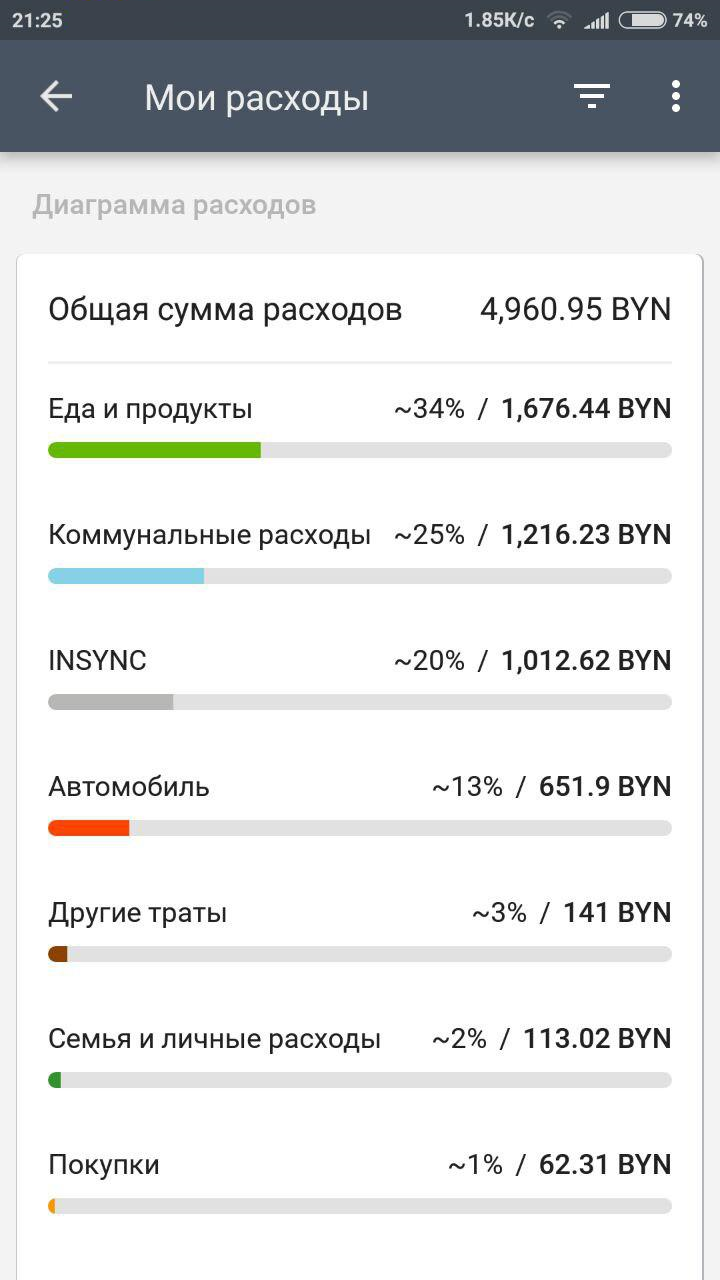
\includegraphics[scale=0.30]{1_2_alfabank.png}
    \caption{Статистика расходов по категориям приложения <<INSYNC.BY>>}
    \label{fig:analysis:analogues:alfabank}
\end{figure}

У описанного решения есть некоторые достоинства:
\begin{itemize}
    \item автоматизированный подсчет и учёт расходов;
    \item для категоризации расходов не требуются действия со стороны пользователя, достаточно производить оплату банковской картой.
\end{itemize}

Однако, несмотря на эти плюсы, у такого подхода есть ряд ощутимых недостатков:
\begin{itemize}
    \item приложения такого типа привязаны к конкретному банку и, соответственно, учитывают расходы только при платежах с карт этого банка;
    \item отсутствие возможности учёта наличных денег;
    \item нет возможности самому контролировать категории расходов в силу того, что категории определяются автоматически исходя из типов заведений, в которых был произведен платеж;
    \item нет возможности определять категории доходов.
\end{itemize}

Описанный выше тип программных средств является быстрым решением, не требующим особых усилий для внедрения в повседневную жизнь, но в то же время не позволяет в полной мере вести учёт и анализ персонального бюджета.

Помимо этого для учёта персонального бюджета существуют программные решения на базе существующих приложений.
Например, в качестве платформы для таких решений может выступать приложение для обмена мгновенными сообщениями <<Telegram>>.
Для платформы разрабатывается \emph{бот} -- программное средство, развернутое на удаленном сервере, которое выполняет роль виртуального собеседника, выполняя действия в ответ на определенные команды пользователя~\cite{telegram_bots}.

Одно из решений для учёта персонального бюджета на базе приложения <<Telegram>> -- бот <<Greenz>> от разработчика ООО <<Простое решение>>.
Поддерживается работа со счетами и бюджетом, категориями расходов и доходов.
Он позволяет фиксировать доходы, все расходы по категориям трат, рассчитывать сумму, которую стоит ежедневно тратить, чтобы не превысить свой месячный бюджет, а если он всё же будет превышен, то бот расскажет, в каких именно категориях был допущен перерасход.
Все данные заносятся в Google-таблицу, которую позже можно анализировать вручную.

У данного подхода по учёту персонального бюджета есть ряд преимуществ по сравнению с обычным мобильным приложением:
\begin{itemize}
    \item на разработку бота требуется куда меньше времени и, соответственно, денег в силу того, что всю инфраструктуру для отображения информации и некоторые другие возможности предоставляет платформа;
    \item <<Telegram>> существует на всех основных мобильных и настольных операционных системах, что позволяет сократить расходы на создание, тестирование и распространение собственного приложения, за исключением непосредственной функциональности бота.
\end{itemize}

Тем не менее, программные средства на базе других приложений имеют список недостатков:
\begin{itemize}
    \item интерфейс ограничен только текстовыми сообщениями, что не позволяет организовать быстрый и удобный доступ ко всем доступным функциям;
    \item работа с приложением невозможна без соединения с интернетом в силу того, что программное средство на самом деле выполняется на удалённом сервере, а не на мобильном устройстве;
    \item работа приложения напрямую зависит от работы и доступности платформы, таким образом в случае отказа платформы недоступным будет и приложение.
\end{itemize}

Также для рассмотрения было выбрано несколько различных мобильных приложений, имеющих более расширенные возможности для учёта персонального бюджета.

Первое из таких приложений -- <<Money Lover -- Менеджер Расходов>> от разработчика Finsify.
Приложение является продвинутым инструментом для учета личных финансов.
Приложение имеет следующие преимущества:
\begin{itemize}
    \item возможность установить лимит затрат и, когда он будет исчерпан, будут появляться уведомления, что больше тратить нельзя;
    \item в приложении присутствует большой выбор категорий по умолчанию, как и возможность создавать свои собственные;
    \item возможность генерирования отчётов о расходах и доходах за произвольный период;
    \item возможность управления долгами;
    \item возможность иметь один аккаунт и приложение сразу на нескольких устройствах: компьютере, планшете и смартфоне.
\end{itemize}

Стоит отметить, что интерфейс <<Money Lover -- Менеджер Расходов>> разработан в соответствии к концепциями Material Design.

Однако большое количество возможностей неизбежно влечёт за собой такие недостатки, как перегруженность пользовательского интерфейса, наличие рекламных баннеров (рисунок~\ref{fig:analysis:analogues:money_lover}), которые закрывают до 15\% рабочего пространства, что осложняет быструю работу с приложением.
Ещё одной особенностью приложения является необходимость регистрации в приложении для работы даже в режиме без соединения с сетью.
Кроме того, приложение достаточно плохо русифицировано, как это можно видеть в списке стандартных категорий (см. рисунок~\ref{fig:analysis:analogues:money_lover}б).

Мобильное приложение <<Транжира -- учет финансов>> от разработчика Worms Studio является ещё одним популярным инструментом для учета личных финансов.
Оно позволяет добавлять доходы и расходы, использовать основную функциональность без авторизации и составлять аналитические отчеты.
Приложение является простым в использовании, ориентированным на быстрый учёт доходов и расходов (главный экран приложения позволяет сразу ввести сумму очередной транзакции), качественно русифицировано и имеет веб-версию.
Однако данное решение не позволяет переносить остатки бюджетов, дублировать транзакции и добавлять к ним теги, геометки и фото.
Кроме этого, большинство функций, необходимых для основательного учёта персонального бюджета, недоступны для бесплатной версии приложения.
Среди таких функций:
\begin{itemize}
    \item наличие множественных счетов;
    \item управление несколькими валютами;
    \item возможности планирования бюджета по категориям.
\end{itemize}

\begin{figure}[h]
    \centering
    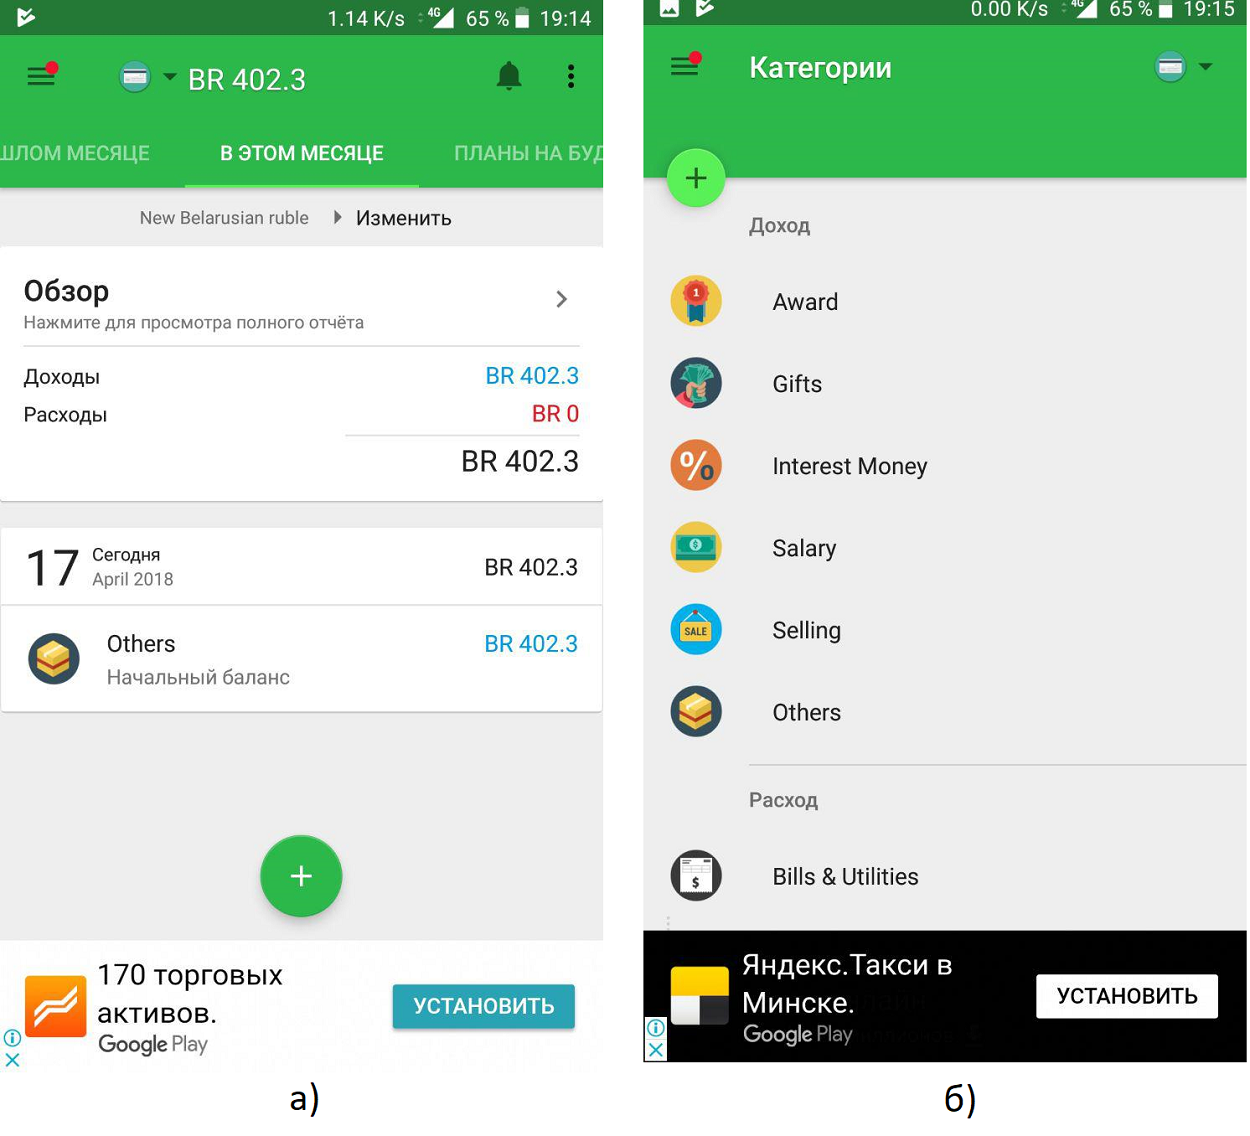
\includegraphics[scale=0.32]{1_2_money_lover.png}
    \caption{Некоторые экраны приложения <<Money Lover -- Менеджер Расходов>>: а) -- главный экран; б) -- меню категорий}
    \label{fig:analysis:analogues:money_lover}
\end{figure}

Отсутствие множественных счетов не позволяет контролировать различные места расположения денег, например наличные деньги и банковская карта.
К тому же нет возможности реализовать какую-либо из описанных в предыдущем разделе методик финансового планирования.

Классическим приложением по учёту персонального бюджета является приложение <<Семейный бюджет>> от разработчика maloii, которое представлено на рисунок~\ref{fig:analysis:analogues:family_budget}.
Приложение предоставляет возможности по управлению счетами и категориями генерации отчётов, а также поддерживает древовидную структуру категорий и мультивалютные счета, что помогает легче структурировать транзакции.

Транзакции в приложении разделены на две группы: доходы и расходы.
Каждая группа представлена в отдельной вкладке.
С первого взгляда такое решение достаточно очевидно -- данные виды транзакций противоположны и собирать их нелогично.
Однако с другой стороны у такого решения имеется ряд недостатков:
\begin{itemize}
    \item нет наглядного представления о всех транзакциях за день;
    \item нельзя посмотреть относительные траты за день (общую сумму всех расходов с учётом доходов);
    \item переводы между двумя счетами нельзя однозначно отнести к какой-либо из транзакций, поэтому в приложении они отображаются сразу в двух вкладках, в расходах -- как расход на счёте-отправителе, в доходах -- как доход для счёта-получателя.
\end{itemize}

Описанные недостатки в некоторой мере понижают наглядность и удобство использования.

Также стоит отметить, что внешний вид приложения устарел и не соответствует рекомендациям Material Design.

\begin{figure}[h]
    \centering
    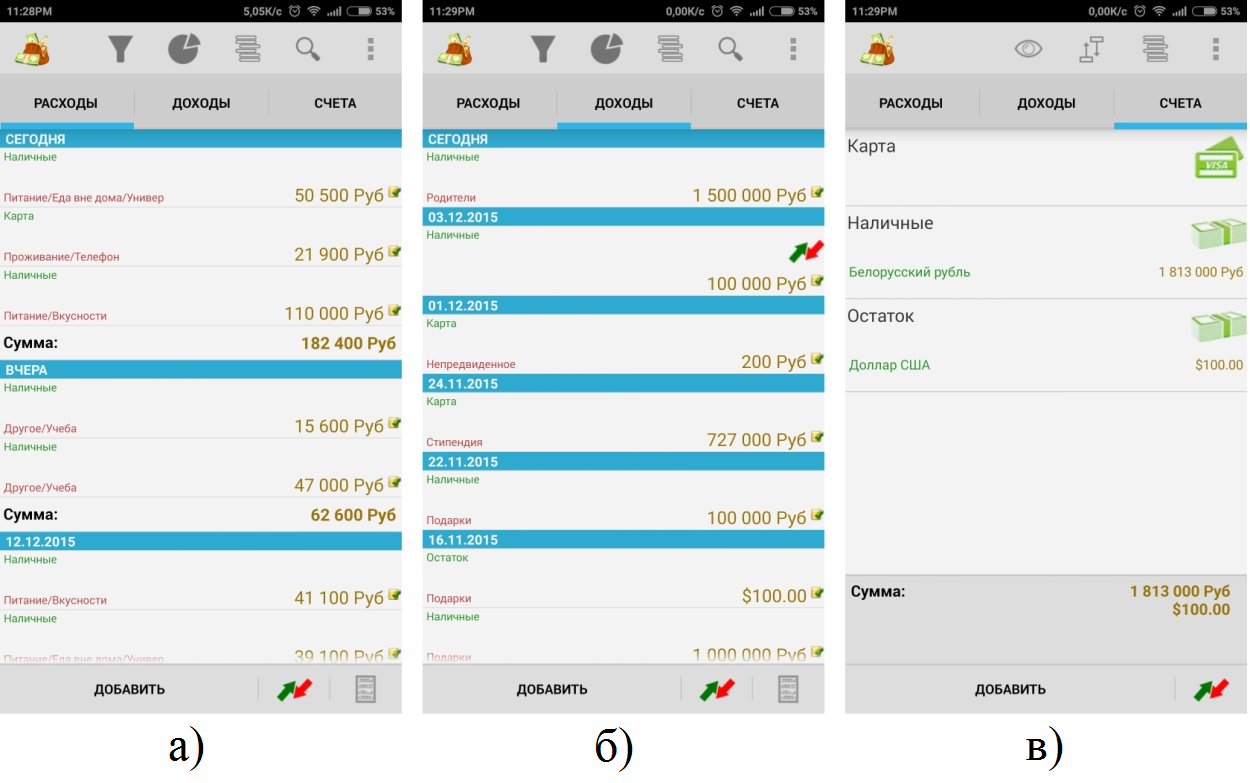
\includegraphics[scale=0.95]{1_2_family_budget.png}
    \caption{Главные экраны приложения <<Семейный бюджет>>:\linebreakа) -- вкладка <<Расходы>>, б) -- вкладка <<Доходы>>, в) -- вкладка <<Счета>>}
    \label{fig:analysis:analogues:family_budget}
\end{figure}


Описанные в данном разделе программные решения по учёту персонального бюджета являются лишь частью всего множества и многообразия существующих прототипов и аналогов в данной области.
Данный анализ позволит сформировать оптимальные функциональные требования для проектируемого программного средства, учитывая преимущества и недостатки других решений, чтобы занять свою область рынка.

\subsection{Требования к проектируемому программному средству}
\label{sec:analysis:specification}

По результатам изучения предметной области, анализа литературных источников и обзора существующих систем-аналогов сформулируем требования к проектируемому программному средству.

\subsubsection{} Назначение проекта
\label{sec:analysis:specification:purpose}

Назначением проекта является разработка программного средства для платформы \andro, упрощающем основные задачи по учёту персонального бюджета.

\subsubsection{} Основные функции
\label{sec:analysis:specification:functions}

Программное средство должно поддерживать следующие основные фун\-к\-ции:

\begin{enumerate}
    \item Использование нескольких валют.
    \item Управление сущностями:
    \begin{enumerate}
        \item категорий расходов и доходов;
        \item счетов;
        \item транзакций.
    \end{enumerate}
    \item Отображение списков:
    \begin{enumerate}
        \item транзакций по дням;
        \item счетов;
        \item категорий по типу.
    \end{enumerate}
    \item Расчёт и отображение:
    \begin{enumerate}
        \item статистики по категориям;
        \item сводных значений по счетам.
    \end{enumerate}
\end{enumerate}

\subsubsection{} Требования к составу и параметрам технических и программных средств
\label{sec:analysis:specification:minimal_requirements}

Одним из важнейших факторов проектирования программного средства для платформы \andro является выбор минимальной версии операционной системы.
Данный параметр определяет соотношение между охватом аудитории и доступными средствами для разработки.
Согласно статистике использования различных версий операционных систем на \andro-устройствах и учитывая тот факт, что каждая последующая версия позволяет выполнять приложения предыдущих версий, программное средство, разработанное для версии 4.4 охватывает около 95\% всех устройств на данной платформе~\cite{android_dashboard}.

Исходя из этого, а также исходя их средних технических характеристик современных мобильных устройств, проектируемое программное средство должно функционировать на устройстве со следующими минимальными характеристиками:
\begin{itemize}
    \item версия операционной системы \andro 4.4 или выше;
    \item тактовая частота процессора от 2 ГГц или более;
    \item оперативная память 2 Гб или более;
    \item диагональ дисплея 4.5 дюймов или более.
\end{itemize}

\subsubsection{} Требования к входным данным
\label{sec:analysis:specification:inputs}

Входные данные для программного средства должны быть представлены в виде вводимого пользователем с помощью клавиатуры текста и выбора доступных опций пользовательского интерфейса.

Должны быть реализованы проверки вводимых данных на корректность с отображением информации об ошибках в случае их некорректности.

\subsubsection{} Требования к выходным данным
\label{sec:analysis:specification:outputs}

Выходные данные программного средства должны быть представлены посредством отображения информации с помощью различных элементов пользовательского интерфейса.

\subsubsection{} Обоснование выбора языка и сред разработки
\label{sec:analysis:specification:lang_rationale}

В качестве языка программирования был выбран язык \emph{\kt} -- лаконичный, безопасный и прагматичный язык, совместимый с языком программирования Java.
Его можно использовать практически везде, где применяется Java: для разработки серверных приложений, приложений для платформы \andro и многого другого.
\kt прекрасно работает со всеми существующими библиотекам и фреймворками, написанными на Java, не уступая последнему в производительности~\cite{kotlin_in_action}.
Данный язык был представлен как \emph{официальный} язык разработки для платформы \andro 17 мая 2017 года~\cite{kotlin_and_android}.

Основные преимущества языка \kt~\cite{kotlin_doc}:
\begin{itemize}
  \item краткость -- конструкции и возможности языка разрабатывались с целью уменьшить 
  количество кода, но при этом не уменьшая читаемости этого кода;
  \item поддержка защиты от нулевого указателя на уровне языка;
  \item полная совместимость с языком программирования Java, что позволяет использовать
  весь набор библиотек и технологий, накопленных за долгое время существования Java;
  \item возможность расширять библиотеки, не изменяя их код, что позволяет дописывать необходимую 
  функциональность без нарушений каких-либо лицензий либо поиска исходных кодов уже 
  скомпилированных библиотек;
  \item мультипарадигмальность -- на языке \kt можно писать код как в процедурном стиле, так и в
  объектно-ориентированном, а также благодаря поддержке функций высшего порядка можно 
  писать код и в функциональном стиле.
  Сочетание лучших качеств у каждого из этих стилей позволяет разрабатывать приложения быстро и эффективно.
\end{itemize}

Таким образом, язык программирования \kt позволяет использовать всю существующую кодовую базу языка \emph{Java} при всей своей лаконичности и простоте, что сильно повышает скорость разработки.

Основной интегрированной средой разработки была выбрана \emph{Android Studio}. Она является официальной средой разработки для платформы проектируемого программного средства~\cite{android_studio}. 

Android Studio предоставляет множество функций, которые значительно упрощают и ускоряют разработку приложений:
\begin{itemize}
    \item расширенный редактор макетов, способность работать с UI компонентами с помощью манипуляций мышью, функция предпросмотра макета на нескольких конфигурациях экрана;
    \item различные виды сборок и генерация нескольких выполняемых файлов приложения;
    \item статический анализатор кода, позволяющий находить проблемы производительности, несовместимости версий и другое;
    \item шаблоны основных макетов и компонентов \andro.
\end{itemize}
